\section{Estado del Arte}
En la actualidad, uno de los aspectos vitales y en crecimiento está constituido por las tecnologías 
de la información, esta apoya la toma de desiciones gerenciales en empresas para agilizar procesos y 
lograr una mejor colaboración entre grupos de trabajo. 
Si bien lo anterior es un punto importante para las empresas la forma en que las personas 
interactúan entre sí y con las organizaciones se ha visto alterada con el surgimiento de Internet y 
de los smartphones.\cite{TI}

Ahora revisaremos los acontacemientos más importantes que fueron un punto clave en la evolución
de los teléfonos a los smartphone.

En 1993 IBM creó el primer smartphone. Lo llamo Simon. Fue el primer smartphone en integrar una 
pantalla táctil. Simon sería el precursor para los smartphones actuales.\cite{Simon}

En 1996 Nokia crea el primer smartphone, Nokia Communicator 9000, con acceso a la web ya  que 
integraba un básico navegador web.\cite{Nokia}

En el año 2007, con el lanzamiento del primer iPhone por parte de Apple se revolucionó el mercado 
de la telefonía móvil y por tanto, muy ligado a él, el de las aplicaciones móviles.
En 2008 se lanza al mercado el primer smartphone con sistema operativo Android. Es en este mismo año 
en el que aparece la primer tienda de aplicaciones de Apple: AppStore. Un año después sale Android 
Market. \cite{Rioja}

Android, en 2017 ha logrando casi un 81.7 por ciento del mercado global, seguido muy distantemente por iOS, 
que casi alcanzó un 12 por ciento en el segundo trimestre del mismo año.\cite{IDC}

Se han desarrollado una gran gama de aplicaciones para smartphone. Hay aplicaciones 
para entretenimento, para conocer personas, para espionaje, para comunicarse a través de mensajes, 
entre muchas otras.[PlayStore] Existe un ramo de las aplicaciones móviles diseñado especificamente para 
brindar información acerca de como desplazarse y/o consultar sitios de interés ya sea dentro de una ciudad 
o un centro comercial. Algunos ejemplos son Google maps, waze, foursquare, 






Hemos visto grandes cambios -- y rumores -- en los últimos meses, incluyendo el primer celular desarrollado 
por Google, la llegada del nuevo asistente virtual, Google Assistant, y los rumores del proyecto llamado 
Andromeda.

Te guste o no Android, es claro el celular que usas o vayas a usar en un futuro haya sido influenciado de 
una u otra manera por este sistema operativo. Después de todo, Android es el más popular del mundo móvil, 
logrando casi un 88 por ciento del mercado global, seguido muy distantemente por iOS, que casi alcanzó un 
12 por ciento en el segundo trimestre del año, según la firma de investigación IDC.[\url{https://www.cnet.com/
es/noticias/android-2017-futuro-novedades-android-8/}]

La plataforma de Android es el producto de la Open Handset Alliance, un grupo de organizaciones que 
colaboran para desarrollar un teléfono móvil mejor. El grupo, dirigido por Google, incluye operadores de 
móviles, fabricantes de dispositivos de auricular, fabricantes de componentes, proveedores de plataformas y 
soluciones de software y compañías de marketing. Desde una perspectiva de desarrollo de software, Android 
está perfectamente en el centro del mundo de código abierto. [\url{https://www.ibm.com/developerworks/ssa/
library/os-android-devel/index.html}]

La diferencia de Android con respecto a todos los sistemas operativos  es que es un software de código 
abierto, no cerrado. El usuario no tiene que conocer esta característica pero es importante de cara al 
mercado.


Un software de código abierto es gratis y accesible a todo el mundo. Esto es especialmente útil para los 
desarrolladores, quienes pueden experimentar y probar, mientras que cada fabricante puede introducir sus 
particularidades. 


En la actualidad las escuelas estan dando prioridad a laa tecnologia de las app, aprovechando que casi 
todos los estudiantes poseen un telefono inteligente.


La mayoria de las aplicaciones moviles en el ambito de la educacion superior se desarrollan para que el 
alumno pueda estar informado y en contacto con su situación academica de su escuela.

Estas apps tienen diferentes caracteristicas cada una las cuales menionaremos en este apartado.

Esta secciíon permitirá comparar trabajos o sistemas de otras escuelas que actualmente se encuentran en 
funcionamiento y disponibles en tiendas de aplicaciones.

Con esto se pretende ver que existe en el mercado y con que cuenta cada universidad, asi como en que se 
diferencia nuestro sistema de otros.
\url{http://noticias.universia.es/vida-universitaria/noticia/2012/05/30/937907/apps-revolucionan-formacion-universitaria.html}

Una de las aplicaciones encontradas es la siguiente:
\pagebreak
\subsection{Red Anáhuac}

\begin{figure}[htbp!]
	\centering
		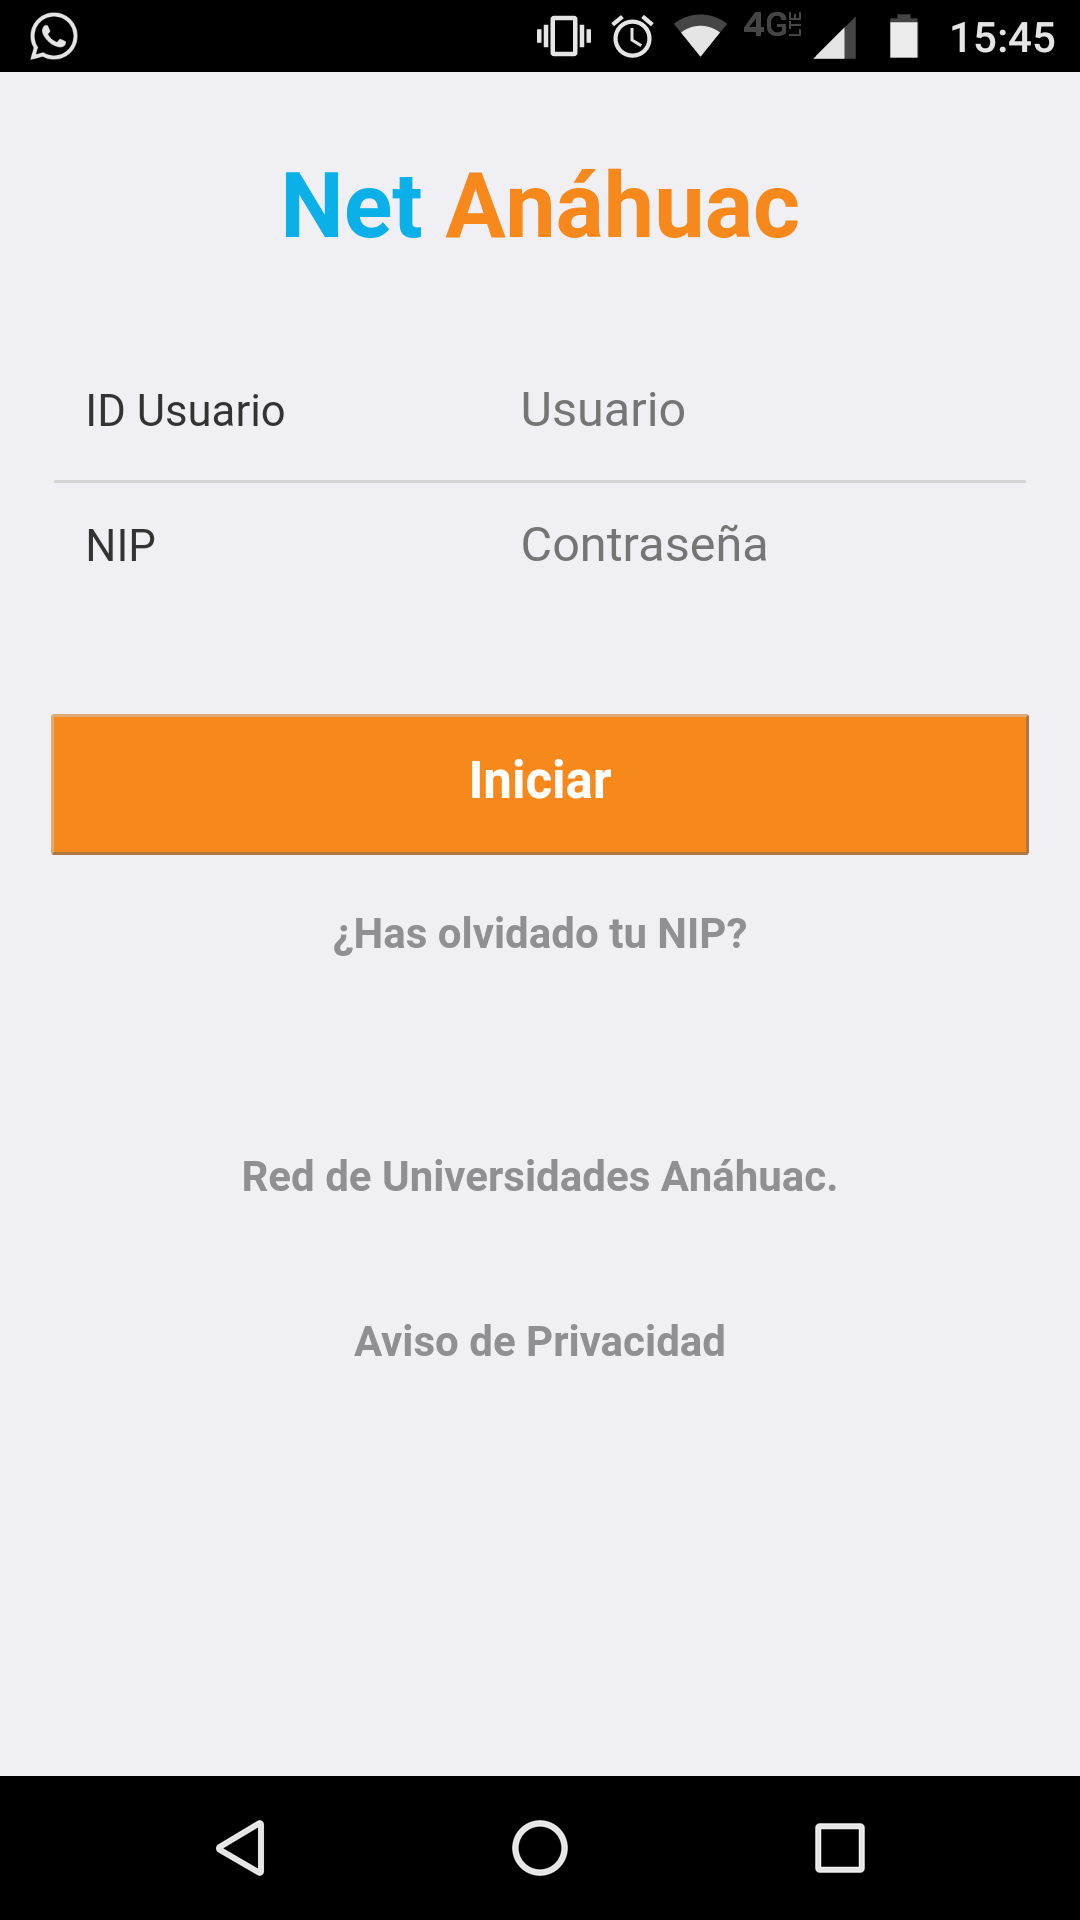
\includegraphics[width=0.3\textwidth]{estado_arte/fotosarte/4}
	\caption{Pagina Inicial NetAnahuac.}
	%\caption{Diseño inconcluso de la base de datos.}
\end{figure}

Aplicación NetAnahuac, esta aplicación esta hecha para la Universidad Anáhuac, es una aplicación que conecta a todos los usuarios de las escuelas de la Anahuac en toda la Republica,
Net anahuac App se puede consultar en cualquier momento y en cualquier lugar.
El estudiante puede obtener información precisa y actualizada.
Sólo necesita usar ID y PIN de Intranet Anáhuac, el mismo que se utiliza comúnmente en el sistema institucional.
Ofreciod por: Fomento e Investigación Integral S.C.
Completa suite de Servicios Academicos y Financieros para la red de Universidades Anáhuac en Mexico


% \begin{table}[!htb]
%\centering
%\caption{RED ANAHUAC}
%\label{my-label1}
%\begin{tabular}{@{}|c|c|c|@{}}
%\toprule
%Caracteristicas  Academicas                                                                                                                                                                                       & Información Financiera                                                                                            & Otros                                                        \\ \midrule
%\begin{tabular}[c]{@{}c@{}}-Busqueda de Cursos\\ -Cursos Planeados\\ -Cita de Inscripción\\ -Horario\\ -Perfil\\ -Situación Academica\\ -Calificaciones Parciales\\ -Historia Academica\\ -Mi Avance\end{tabular} & \begin{tabular}[c]{@{}c@{}}-Estado de Cuenta\\ -Credito Educativo\\ -Apoyo Financiero\\ -Retenciones\end{tabular} & \begin{tabular}[c]{@{}c@{}}-Noticias\\ -Eventos\end{tabular} \\ \bottomrule
%\end{tabular}
%\end{table}

Esta aplicación se encuentra disponible para IOS y Android, 

\pagebreak
\subsection{MIT MOBILE}

El MIT Mobile Experience Lab utiliza dispositivos móviles personales para desbloquear el potencial en el mundo físico que nos rodea. Buscamos reinventar radicalmente y diseñar creativamente conexiones entre personas, información y lugares.[REFERENCIA]

\begin{figure}[htbp!]
		\centering
			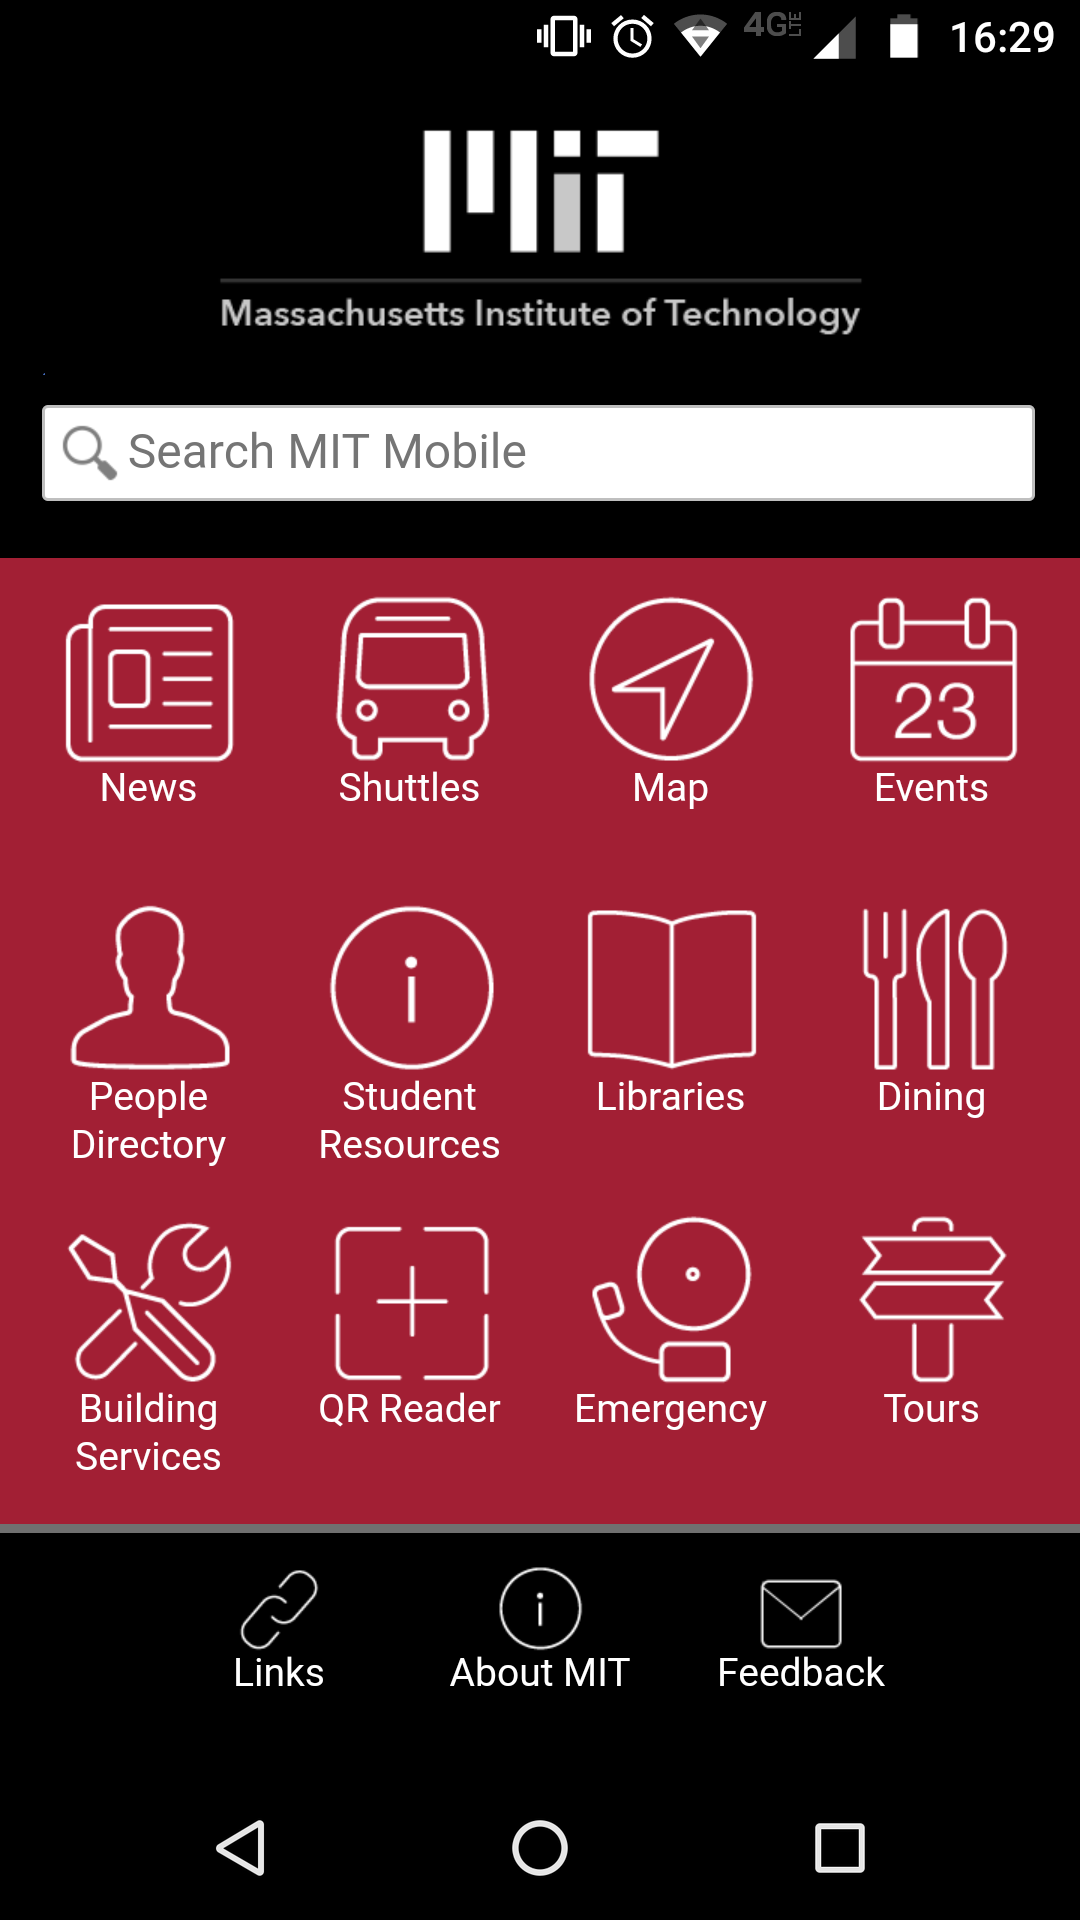
\includegraphics[width=0.3\textwidth]{estado_arte/fotosarte/5}
		\caption{Pagina Inicial MIT MOBILE.}
		\end{figure}
		
 \begin{table}[!htb]
\centering
\caption{MIT MOBILE}
\label{my-label4}
\begin{tabular}{|c|}
\hline
Caracteristicas                                                                                                                                                                                                                                                    \\ \hline
\begin{tabular}[c]{@{}c@{}}-\\ Noticias del Campus,\\ Busqueda del mapa del campus,\\ Calendario de Eventos,\\ Busqueda de Directorio,\\ Informacion sobre el MIT\\ Informacion sobre campus de emergencias\\ Menu de comidas\\ Reportes\\ Scanner QR\end{tabular} \\ \hline
\end{tabular}
\end{table}
	
	\pagebreak
\subsection{CONEXION UVM}	

Solución móvil de la UVM que soporta el proceso de toma y consulta de asistencia, así como la consulta de calificaciones en línea de los alumnos en curso; además de proveer un medio de comunicación directa entre la comunidad estudiantil, docente y administrativa a través del envío de notificaciones, encuestas y mensajes.


\begin{figure}[htbp!]
		\centering
			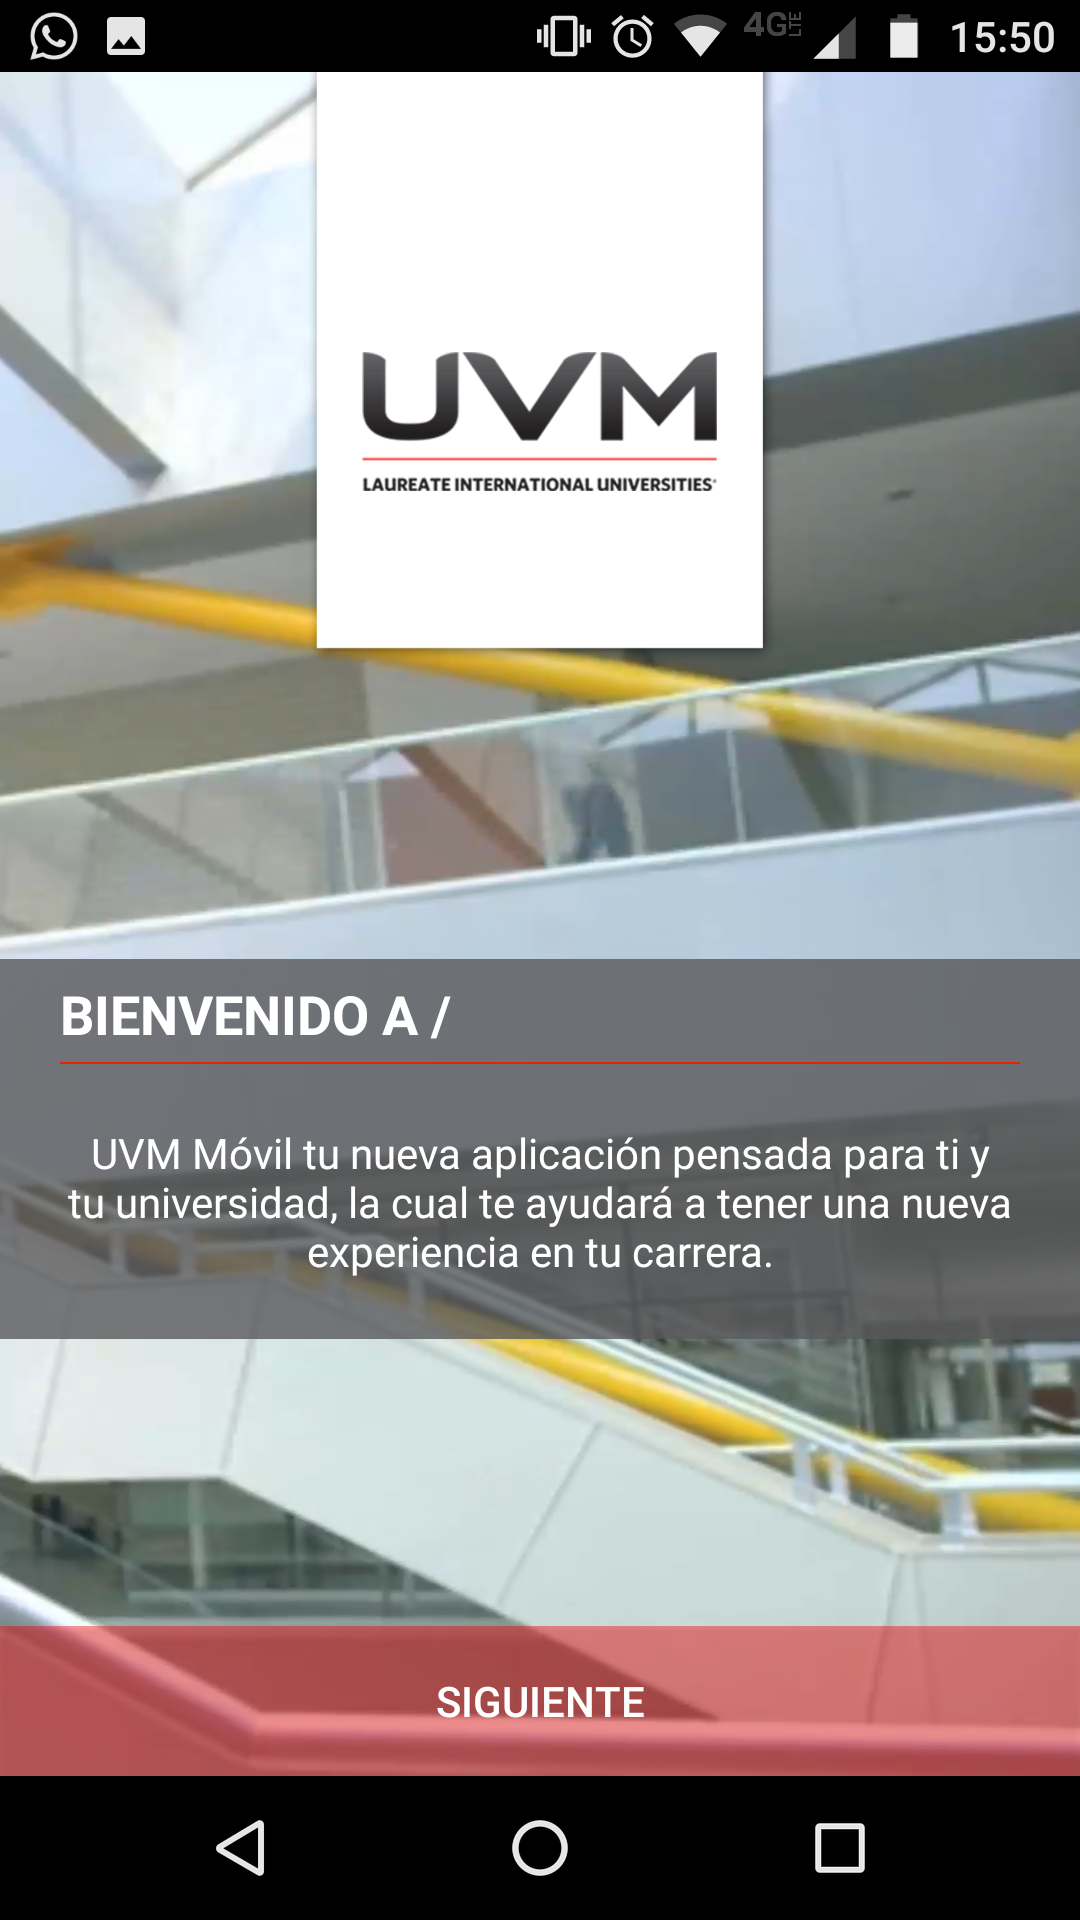
\includegraphics[width=0.3\textwidth]{estado_arte/fotosarte/6}
		\caption{Pagina Inicial Conexion UVM.}
		\end{figure}

 \begin{table}[!htb]
\centering
\caption{CONEXIÓN UVM}
\label{my-label2}
\begin{tabular}{|c|}
\hline
Caracteristicas                                                                                                                                                                                         \\ \hline
\begin{tabular}[c]{@{}c@{}}Consultade Asistencia\\ Consulta de Calificaciones\\ Medio,de comunicación entre la comunidad estudiantil\\ Notificaciones\\ Comunicación,estudiante y profesor\end{tabular} \\ \hline
\end{tabular}
\end{table}

Disponible para IOS Y ANDROID
\pagebreak
\subsection{IBERO MOVIL}

Ibero Móvil es tu aplicación de la Universidad Iberoamericana Ciudad de México, para acceder a tu información académica, de estados de cuenta, y realizar la reinscripción de tus materias. Fue realizada por la Dirección de Informática y Telecomunicaciones.

\begin{figure}[htbp!]
		\centering
			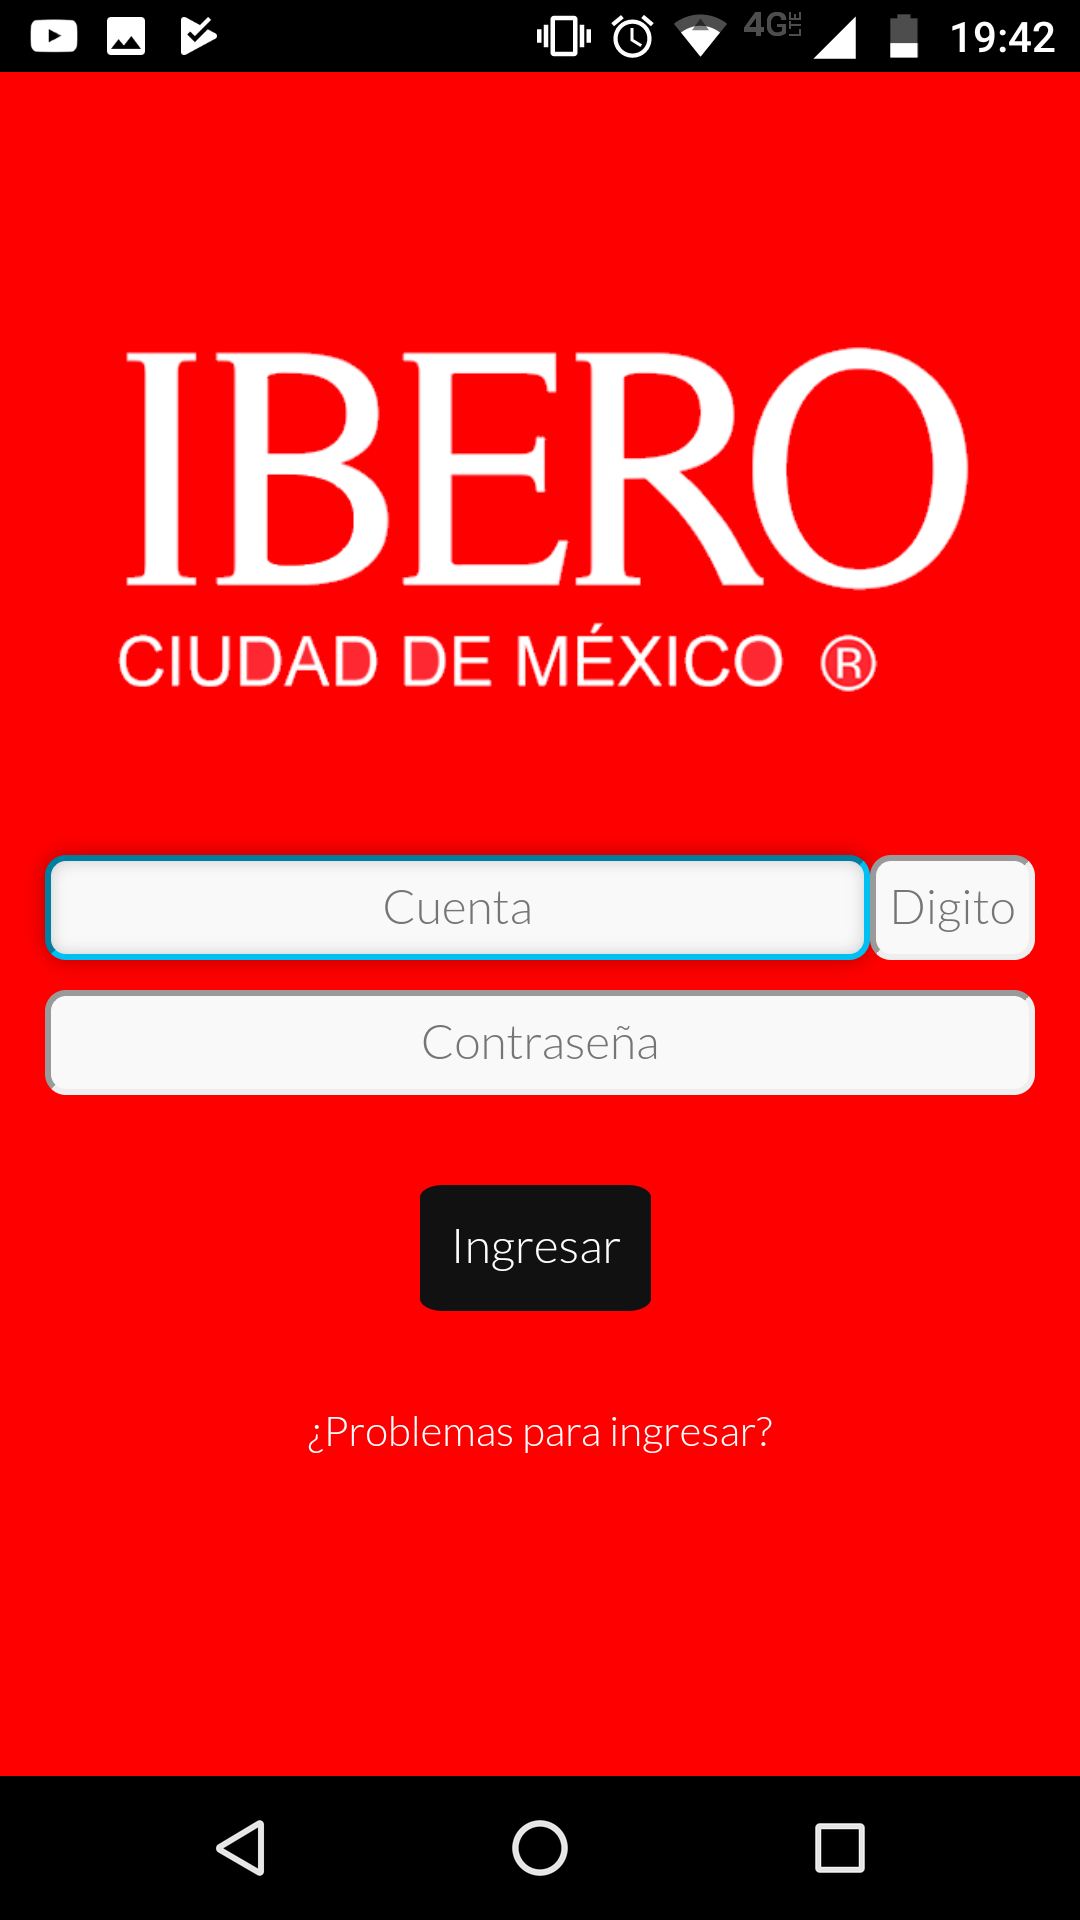
\includegraphics[width=0.3\textwidth]{estado_arte/fotosarte/ibero}
		\caption{Pagina Inicial Conexion UVM.}
		\end{figure}
		
		
 \begin{table}[!htb]
\centering
\caption{IBERO MOVIL}
\label{my-label3}
\begin{tabular}{|c|}
\hline
Caracteristicas                                                                                                                                                                                                   \\ \hline
\begin{tabular}[c]{@{}c@{}}-Busqueda de Cursos\\ -Cursos Planeados\\ -Cita de Inscripción\\ -Horario\\ -Perfil\\ -Situación Academica\\ -Calificaciones Parciales\\ -Historia Academica\\ -Mi Avance\end{tabular} \\ \hline
\end{tabular}
\end{table}
	
	
	Tambien en la ESCOM se han desarrolado ciertas aplicaciones para el uso de los estudiantes, aqui mostramos algunas:
	
	\subsection{MANIFEST ESCOM}
	
	Aplicación para la difusión de la información en la Escuela Superior de Cómputo
	
	Manifest es una aplicación diseñada para mantenerte al tanto de los últimos acontecimientos que ocurren en la Escuela Superior de Cómputo, y asi seguir los temas de interes para la comunidad
	
	 \begin{table}[!htb]
\centering
\caption{MANIFEST ESCOM}
\label{my-label5}
\begin{tabular}{|c|}
\hline
Caracteristicas                                                                                            \\ \hline
\begin{tabular}[c]{@{}c@{}}-Eventos\\ -Cursos\\ -Convocatorias\\ -Noticias\\ -Avisos Urgentes\end{tabular} \\ \hline
\end{tabular}
\end{table}
	
	\subsection{ESCOMobile}
	ESCOMobile es nuestra propuesta para una herramienta movil para los alumnos de la ESCOM
	
 \begin{table}[!htb]
\centering
\caption{ESCOMobile}
\label{my-label6}
\begin{tabular}{|c|}
\hline
Caracteristicas                                                                                                                                                                                                           \\ \hline
\begin{tabular}[c]{@{}c@{}}-Horarios de clase\\ -Registro Alumnos y Profesores\\ -Eventos\\ -Citas\\ -Mapa de la ESCOM\\ -Cursos\\ -Perfiles\\ -Busqueda de Profesores\\ -Notificaciones\\ -Acceso Invitados\end{tabular} \\ \hline
\end{tabular}
\end{table}